\documentclass[useAMS,usenatbib,fleqn]{mn2e}
\usepackage{amsmath}
\usepackage{amssymb}
\usepackage{graphicx}
\usepackage{caption}
\usepackage{subcaption}
  
\captionsetup{compatibility=false}

\title[Photometric Redshift Estimation]{Photometric Redshift Estimation}
\author[Almosallam et al.]
{\parbox{\textwidth}{Author1,$^1$\thanks{E-mail: ibrahim.almosallam@some.ox.ac.uk} 
Author2,$^{2}$ etc.
} 
\vspace{0.4cm}\\ 
\parbox{\textwidth}{
$^1$Oxford Astrophysics, Department of Physics, Keble Road, Oxford, OX1 3RH, UK\\
$^2$Other institution \\
}}


\begin{document}

\date{\today}

\pagerange{\pageref{firstpage}--\pageref{lastpage}} \pubyear{2015}

\maketitle

\label{first page}

\begin{abstract}
In this study, a novel sparse regression model for photometric redshift estimation is presented which directly target the requirements for the Euclid Space Mission. Data from a synthesised survey was used to train and test the proposed models. We show that approaches which include careful data preparation and model design, a significant improvement can be achieved when compared with several off the shelf machine learning algorithms. Standard implementation of most regression algorithms has as objective the minimisation of the sum of squared errors. This induces a bias in the posterior mean of the output distribution which can be problematic. In this paper we directly optimise the Euclid mission requirement and compare this with other objective functions, such as minimising the maximum error and maximising the number of data points with a predictive error less than a threshold. The results are compared with other popular machine learning algorithms in the field such as ANNz, stableGP and SPGP. The proposed reached a $\Delta z = 0.0085(1+z)$ for a redshift range of $0.2 < z < 2$, exceeding the requirement for the Euclid mission of $\Delta z = 0.05(1+z)$ for the same redshift range.

\end{abstract}

\begin{keywords}
methods: data analysis -- galaxies: distances and redshifts
\end{keywords}

\section{Introduction}
We introduce a novel sparse kernel regression model that greatly reduces the number of bases functions required to model the data. This os achieved this by allowing each kernel to have its own hyper-parameters, governing its shape. This is in contrast to the standard kernel-based model in which a set of global hyper-parameters are optimised. The complexity cost of such a kernel-based regression model is $O(n^{3})$, where $n$ is the number of bases functions. This cubic time complexity arise from the cost of inverting a $n$ by $n$ covariance matrix. In a basic Gaussian Process model (GP) \cite{rasmussen+williams}, seen as a kernel regression algorithm, we may regard the number of bases, $n$, as equal to the number of points in the training set. This renders such an approach unusable for many large-data applications where scalability is a major concern. Much of the work done to make GPs more scalable \cite{sparseGPcitations} is either to make the inverse computation faster or use smaller representative sample to compute the covariance. Examples of the former includes methods such as structuring the covariance matrix such that it is much easier to invert \cite{}, using Toeplitz and Kronecker decomposition for example, or inverse approximation as an optimisation problem \cite{}. To reduce the number of representative points, an $m << n$ subset of the training set can be selected which maximises the accuracy or the numerical stability of the inversion. Alternatively, one may search for "pseudo" points not necessarily present in the training set to use as bases for the covariance matrix such that it maximises the log marginal likelihood \cite{}. The focus in this paper is on sparse GP modelling where we extend the sparse pseudo-point GP using less, but more flexible kernels. Moreover, a weighting scheme is modelled as an integral part of the process to remove, or introduce, any systematic bias to the model. The results are demonstrated on photometric redshift estimation for the Euclid Space Mission. In particular, we use the weighting scheme to remove any distribution bias and introduce a linear bias to directly target the mission's requirement. The proposed approach reached a $\Delta z = 0.0085(1+z)$ on a simulated catalogue, far exceeding the mission's requirement of $\Delta z = 0.05(1+z)$ The paper is organised as follows, a brief introduction to Gaussian Processes for regression and sparse GPs are presented in sections \ref{sec-gaussian-process} and \ref{sec-sparse-gaussian-process},  then the proposed approach is laid out in Section \ref{sec-proposed-approach}. We discuss other objectives that can be useful for other scientific goals in \ref{sec-other-objectives} then the data set description and experiments are provided in Sections \ref{sec-dataset} and \ref{sec-experiment} respectively. We summarise and conclude in Section \ref{sec-conclusion}.

\textit{TO ADD: The contributions of this paper are as follows....}

\section{Gaussian Processes}
\label{sec-gaussian-process}
In many modelling problems, we have little prior knowledge of the explicit functional form of the function which maps our observable variables into the variable of interest. Imposing, albeit sensible, parametric models, such as polynomials, makes a tacit bias. For this reason, much of modern function modelling is performed using \emph{non-parametric} techniques. For regression, the most widely used approach is that of \emph{Gaussian Processes}.
A Gaussian Process is a supervised non-linear regression algorithm that makes few explicit \emph{parametric} assumptions about the nature of the function fit. For this reason, Gaussian Processes are seen as lying within the class of Bayesian non-parametric models. The main underlying assumption in a GP is that the joint probability of the input variable $x$ and the output variable $y$ is a multivariate Gaussian with mean $\mu=\begin{bmatrix} \mu_{x}\\ \mu_{y}\end{bmatrix}$ and covariance $\Sigma=\begin{bmatrix}\Sigma_{xx} & \Sigma_{xy}\\\Sigma_{yx} & \Sigma_{yy} \end{bmatrix}$, where $\Sigma_{xy}=(x-\mu_{x})(y-\mu_{y})^{T}$. The input variables $x$ is an $n$ by $d$ matrix, where $n$ is the number of data points and $d$ is the dimensionality of the input. Without loss of generality, the output variable $y$ is assumed to be a vector of length $n$ of target outputs but the same concept can be applied to multiple variable output.

\begin{equation}
p\left ( x,y\right) \sim \mathcal{N} \left ( \begin{bmatrix}\mu_{x}\\\mu_{y} \end{bmatrix}, \begin{bmatrix}\Sigma_{xx} & \Sigma_{xy}\\\Sigma_{yx} & \Sigma_{yy} \end{bmatrix}\right )
\end{equation}

The mean and covariance of the conditional probability $p(y|x)$ therefore is Gaussian distributed as follows:
\begin{equation}
p(y|x) \sim  \mathcal{N} \left ( \mu_{x}+\Sigma_{yx}\Sigma_{xx}^{-1}\left ( y-\mu_{y}\right ), \Sigma_{yy}-\Sigma_{yx}\Sigma_{xx}^{-1}\Sigma_{xy}\right )
\end{equation}

The calculation can be simplified by subtracting the mean of the input and the output variables and assuming a prior mean $\mu_{x}=\mu_{y}=0$ and $\Sigma_{xy}$ redefined as $xy^{T}$. The conditional probability $p(y|x)$ can then be rewritten as:

\begin{equation}
\label{eq-conditional-zero-mean}
p(y|x) \sim  \mathcal{N} \left ( \Sigma_{yx}\Sigma_{xx}^{-1}y, \Sigma_{yy}-\Sigma_{yx}\Sigma_{xx}^{-1}\Sigma_{xy}\right )
\end{equation}

For the rest of this paper, the prior mean is assumed to be zero unless otherwise stated. So far, it is assumed that no noise exists in our $y$ observations. It can be shown that assuming some noise $\epsilon \sim \mathcal{N}\left(0,\sigma_{n}^{2}\right)$ on the output variable $y$, yields a the following:

\begin{equation}
\label{eq-mean-variance-noise}
p(y|x) \sim  \mathcal{N} \left ( \Sigma_{yx}\left(\Sigma_{xx}+I\sigma_{n}^{2}\right)^{-1}y, \Sigma_{yy}-\Sigma_{yx}\left(\Sigma_{xx}+I\sigma_{n}^{2}\right)^{-1}\Sigma_{xy}+\sigma_{n}^{2}\right )
\end{equation}

For our current definition of the covariance matrix $\Sigma$, the predictive mean is equivalent to a linear regression model, in fact, one can reach the same conclusion by finding the linear regression model that minimizes the sum of squared errors. In other words, the model that minimizes the sum of squared errors also maximizes the probability of the data. For in depth discussion on Gaussian processes and its Bayesian interpretation, the reader is referred to \cite{}.

Since the solution is entirely defined as inner products of the data points, one can utilize the so called ``kernel trick" to learn non-linear models by replacing the covariance matrix $\Sigma$ with a covariance function $K$, where $K_{ij} = k(x_{i},x_{j})$.

The kernel function $k$ is defined such that the matrix $K$ will be a positive definite matrix. The concept behind the kernel trick is to compute the covariance matrix of high dimensional mapping of the input into a higher dimensional space without explicitly mapping them to that space. The choice of kernel is largely a modelling decision based on the definition of similarity for a given application. In this paper, the squared exponential kernel defined in \eqref{eq-squared-exponential} is used but the concepts introduced here applies to any other kernel function.

\textit{COMMENT: in general I think a more full description is needed. Reading the above feels like the choice of kernel is arbitrary}

\textit{TO ADD: explain why the SE is used - what assumptions does it impose and what advantages does it have.}

\begin{equation}
\label{eq-squared-exponential}
k(x_{i},x_{j}) = \sigma^{2} \exp \left ( -\frac{\sum_{k=1}^{d} ( x_{ik}-x_{jk} )^{2}} {2\lambda^{2}} \right )
\end{equation}

The hyper-parameters of the squared exponential kernel $\sigma^{2}$ and $\lambda^{2}$ are called the height variance and characteristic length scale respectively. Together with the noise variance $\sigma_{n}^{2}$ define the set of hyper-parameters for the GP model. The optimal set of hyper-parameters are the set of values that maximizes the probability of the data given the model, which can be achieved by maximizing the log marginal likelihood defined in \eqref{eq-log-marginal-likelihood} 

\begin{equation}
\label{eq-log-marginal-likelihood}
\log\text{ }p(y|x) = -\frac{1}{2}y^{T}\left(K+I\sigma_{n}^{2} \right)^{-1}y-\frac{1}{2} \log\left | K+I\sigma_{n}^{2}\right|-\frac{n}{2}log(2\pi)
\end{equation}

This can be achieved by using a gradient search based optimization by taking the derivative of the log marginal likelihood with respect to each hyper-parameter and following the direction of the gradient.

\section{Sparse Gaussian Process}
\label{sec-sparse-gaussian-process}
Gaussian processes are often described as non-parametric regression models due to the analytical nature of its solution and its use of very limited number of hyper-parameters that live in the kernel. However, GP regression can be viewed as feature transformation methods $x\in \mathbb{R}^{d}:\rightarrow K\in \mathbb{R}^{n}$ parameterized by the data and the kernel function followed by a linear regression, or optimizing the following objective:

\begin{equation}
\label{eq-linear-regression-objective}
f(w)=\frac{1}{2}\left ( Kw-y \right )^{T} \left( Kw-y \right )+\frac{1}{2}\sigma_{n}^{2}w^{T}w
\end{equation}

The feature transformation $K$ is essentially describing each data point by how ``similar" it is to every point in the training set where the similarity measure is defined by the kernel function. Obviously, if two training points are very similar, that will result in very correlated features and thus adding extra computational cost for very little or no added information. Selecting a subset of the training set that maximizes the preserved information is a research question addressed in [x], whereas in [x] the basis functions are treated as an optimization problem rather than a selection problem where their locations are treated as hyper-parameters. The new transformation is now $x\in \mathbb{R}^{d}:\rightarrow K\in \mathbb{R}^{m}$ where $m<<n$ is the number of bases used. The transformation matrix $K$ will therefore be a rectangular $n$ by $m$ matrix and the solution for $w$ in \eqref{eq-linear-regression-objective} is calculated as follows:

\begin{equation}
\label{eq-linear-regression-objective-rectangular}
w = \left(K^{T}K+I\sigma_{n}^{2} \right)^{-1}K^{T}y
\end{equation}

Even though these models improve the computational cost greatly, very little is done to compensate for the reduction in modeling complexity. The selection method is always bounded by the full GP's accuracy. On the other hand, the sparse GP's ability to place the bases freely across the input space does compensate for the bases set size reduction as they can be better positioned to describe the distribution of the data. However, in both cases a global set of hyper-parameters is used for all basis functions therefore limiting the algorithm's capability to model patterns in the data with the number of basis and their locations. Moreover, the objective in \eqref{eq-linear-regression-objective} by definition minimizes the sum of squared errors, therefore for any non-uniformly distributed output, the optimization routine will bias the model towards the mean of the output distribution and to fit the region of space where there is more data.

In the next section, the proposed method is described which address the above issues by defining each basis with its own hyper-parameters to account for variable density and/or pattern across the input space and allows the algorithm to learn more complex models with a fewer number of basis functions. In addition, a weighting mechanism to remove any distribution bias from the model is directly incorporated into the objective.

\section{Proposed Approach}
\label{sec-proposed-approach}

In this paper, we extend the sparse GP approach by modeling each basis with its own set of hyper-parameters, namely the kernel function in \eqref{eq-squared-exponential} is redefined as follows:

\begin{equation}
\label{eq-squared-exponential-extension}
k(x_{i},p_{j}) = e^{-\frac{\left\| x_{i}-p_{j}\right\|^{2}}{2\lambda_{j}^{2}}}
\end{equation}

Where $P=\{p_{j}\}_{j=1}^{m}$ is the set of bases coordinates in $\mathbb{R}^{d}$ and $\lambda_{j}$ is the corresponding length scale for basis $j$. Note that the hyper-parameter $\sigma$ has been dropped, as it interferes with the regularization objective. This can be seen from the final prediction equation $f(x_{i},w)=\sum_{j=1}^{m}w_{j}\sigma_{j}^{2}e^{-\left\| x_{i}-p_{j}\right\|^{2}/2\lambda_{j}^{2}}$, the weights are always multiplied by their associated $\sigma$. Therefore, the optimization process will always compensate for decreasing $w_{j}^{2}$ by increasing $\sigma_{j}^{2}$. Dropping the height variance ensures that the kernel functions do not grow beyond control and delegates learning the linear coefficients and regularization to the weights $w_{j}$. A gradient based optimization is used to find the set of hyper-parameters by computing the derivatives with respect to each variable to compute the search direction, specifically we used a Quasi-Newton optimization using the L-BFGS algorithm \cite{}. The derivative with respect to each length scale and position are provided in equations \eqref{eq-dfdl} and \eqref{eq-dfdp} respectively. 

\begin{subequations}
\begin{align} 
\label{eq-dfdl}
\frac{\partial f(x,w)}{\partial \lambda_{j}} &= \sum_{i=1}^{n}\left(f(x_{i},w)-y_{i}\right)w_{j}K_{ij}\frac{\left\| x_{i}-p_{j}\right\|^{2}}{\lambda_{j}^{3}}\\
\label{eq-dfdp}
\frac{\partial f(x,w)}{\partial p_{jk}} &= \sum_{i=1}^{n}\left(f(x_{i},w)-y_{i}\right)w_{j}K_{ij}\frac{(x_{ik}-p_{jk})}{\lambda_{j}^{2}}
\end{align}
\end{subequations}


Finding the set of hyper-parameters that optimizes the solution, is in effect finding the set of radial bases defined by their positions $p$ and radius $\lambda$ that jointly describes the patterns across the input space, and by parameterizing them differently, the model is more capable to accommodate different regions in the space more specifically. The kernel in \eqref{eq-squared-exponential-extension} can be further extended to, not only model each basis with its own radius $\lambda_{j}$, but also model each one with its own covariance defined by $C_{j}$. This enables the bases to have any arbitrary shaped ellipses given it more flexibility. The kernel in \eqref{eq-squared-exponential-extension} can be extended as follows:

\begin{equation}
\label{eq-squared-exponential-covariance-extension}
k(x_{i},p_{j}) = e^{-\frac{1}{2}\left(x_{i}-p_{j}\right)C_{j}^{-1}\left(x_{i}-p_{j}\right)^{T}}
\end{equation}

To make the optimization process faster and simpler, we define the following variables:

\begin{subequations}
\begin{align} 
\label{eq-error}
E &= \left(f(x,w)-y)\right)w^{T}\\
\label{eq-Cinv}
C_{j}^{-1} &= \Lambda\Lambda_{j}^{T}\\
\label{eq-Delta_j}
\Delta_{j} &= \left(x-\underset{n}{1}p_{j}\right)\\
\label{eq-V_j}
V_{j} &= \Delta_{j}\Lambda_{j}
\end{align}
\end{subequations}

Where $\underset{n}{1}$ denotes a column vector of length $n$ with all elements set to 1. Optimizing with respect to $\Lambda_{j}$ directly ensures that the covariance matrix is positive semi-definite and makes it faster from a computational perspective, as the kernel functions for all the points with respect to a particular basis can be computed more efficiently as follows:

\begin{equation}
\label{eq-squared-exponential-covariance-extension-simplified}
k(x,p_{j}) = e^{-\frac{1}{2}\left(V_{j}\circ V_{j}\right)\underset{d}{1}}
\end{equation}

The symbol $\circ$ denotes the Hadamard product or the element-wise matrix multiplication. The exponent in \eqref{eq-squared-exponential-covariance-extension-simplified} basically reads, square the elements of the matrix $V_{j}$ then compute the sum of each row. This allows for a more efficient computation of the kernel functions for all points in a single matrix operation. The derivatives with respect to each $\Lambda_{j}$ and $p_{j}$ are shown in \eqref{eq-dfdL} and \eqref{eq-dfdP}

\begin{subequations}
\begin{align} 
\label{eq-dfdL}
\frac{\partial f(x,w)}{\partial \Lambda_{j}} &= -\left( \Delta_{j}\circ \left(\left(K_{*,j}\circ E_{*,j}\right)\underset{d}{1}\right) \right)^{T}V_{j}\\
\label{eq-dfdP}
\frac{\partial f(x,w)}{\partial p_{j}} &= \left( K_{*,j}\circ E_{*,j} \right)^{T}V_{j}\Lambda_{j}^{T}
\end{align}
\end{subequations}

Where $K_{*,j}$ is the $j$'th column of matrix $K$, similarly for $E_{*,j}$. The differences between the three approaches using a different number of bases functions are demonstrated on a toy classification example shown in figure \ref{fig-toy-example} and the results are shown in figure \ref{fig-toy-comparison}. The class probability distribution clearly show the advantage of having bases functions with more flexibility. 

\begin{figure}
       \centering
       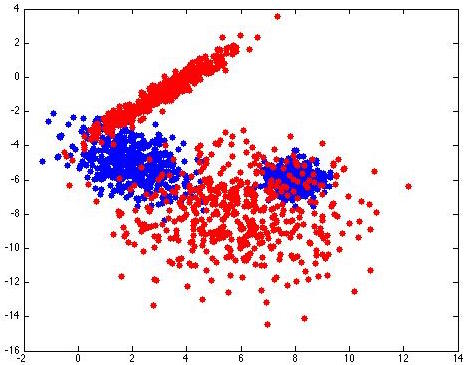
\includegraphics[trim = 25px 12px 10px 10px, clip=true,width=\columnwidth]{clouds.jpg}
        \caption{A toy classification dataset. }       
       \label{fig-toy-example}
\end{figure}

  
\begin{figure*}
        \centering
        \begin{subfigure}[b]{90 px}
                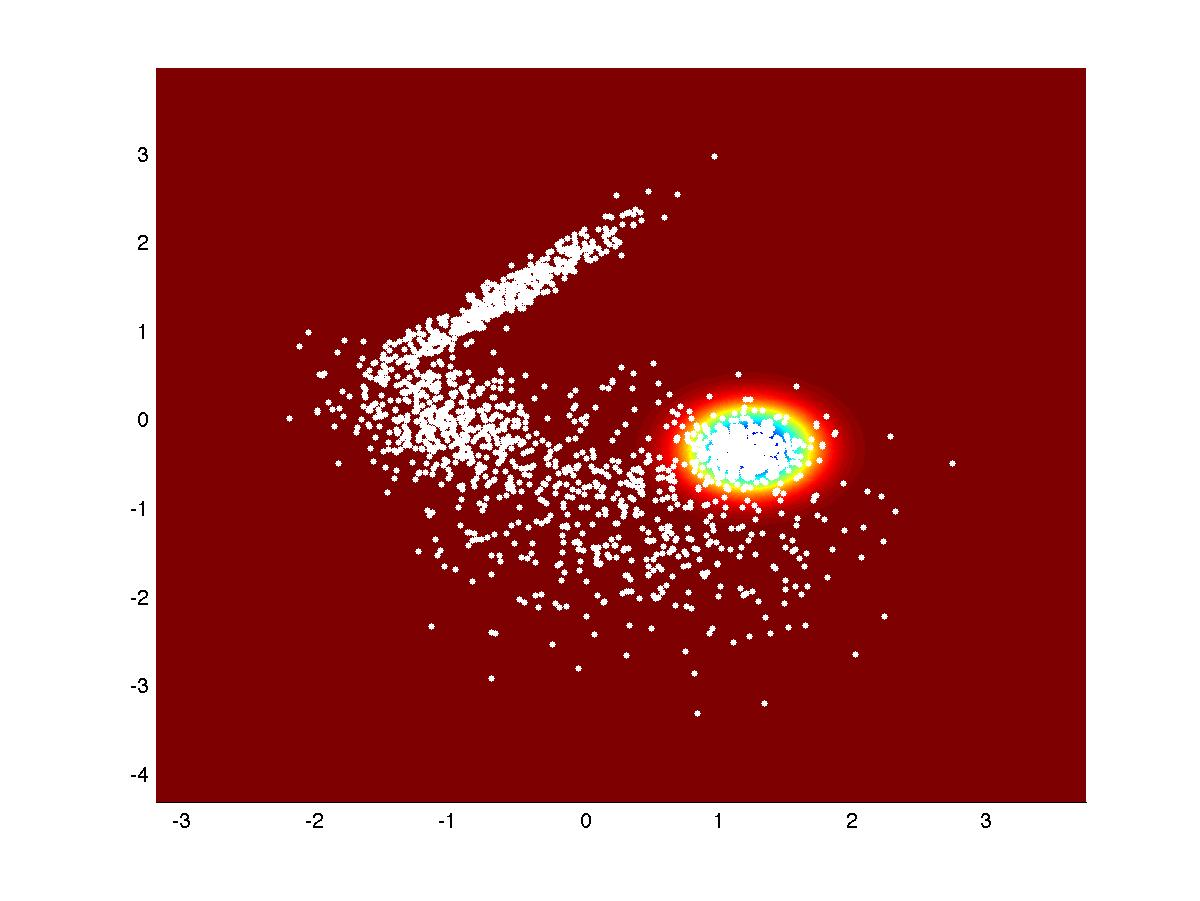
\includegraphics[trim = 150px 100px 150px 70px, clip=true,width=\textwidth]{global1.jpg}
        \end{subfigure}
        ~
         \begin{subfigure}[b]{90 px}
                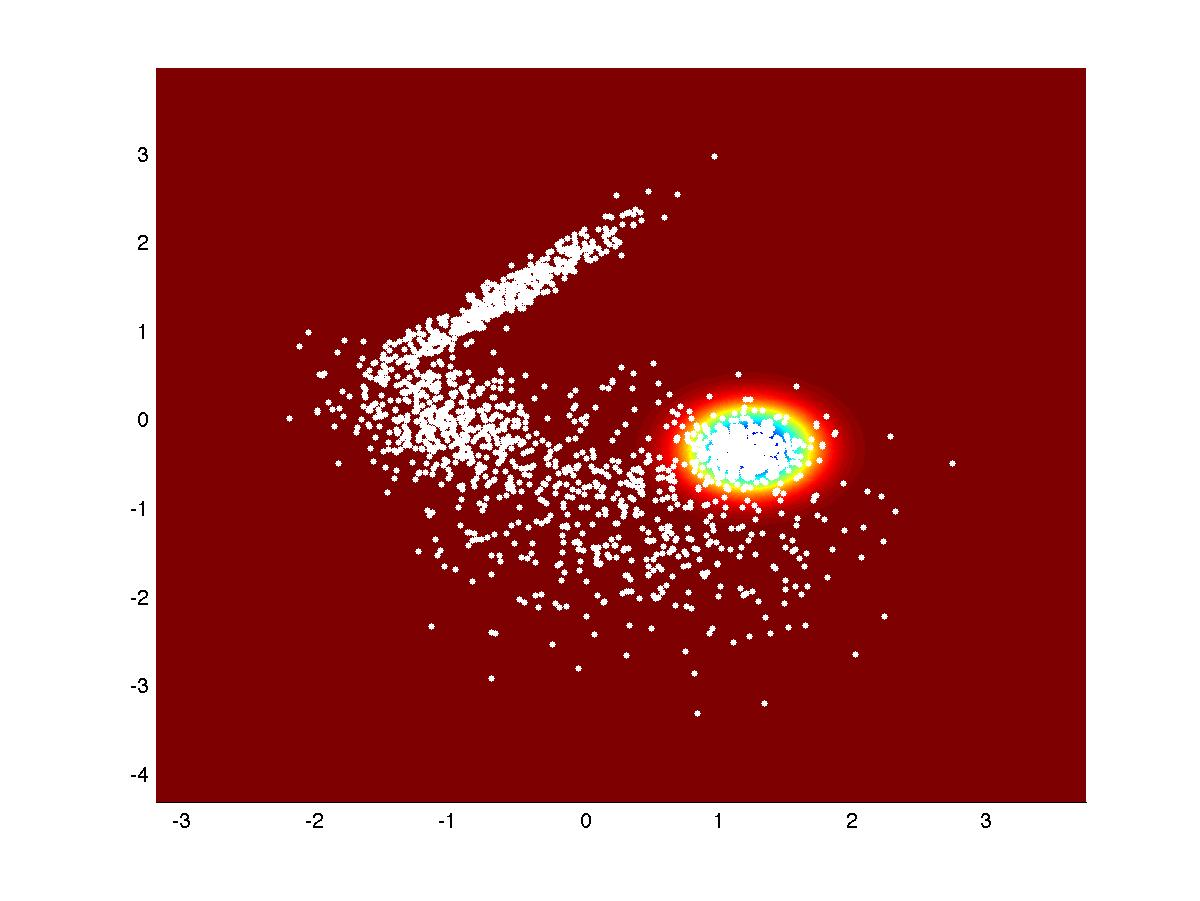
\includegraphics[trim = 150px 100px 150px 70px, clip=true,width=\textwidth]{VL1.jpg}
        \end{subfigure}
        ~
        \begin{subfigure}[b]{90 px}
                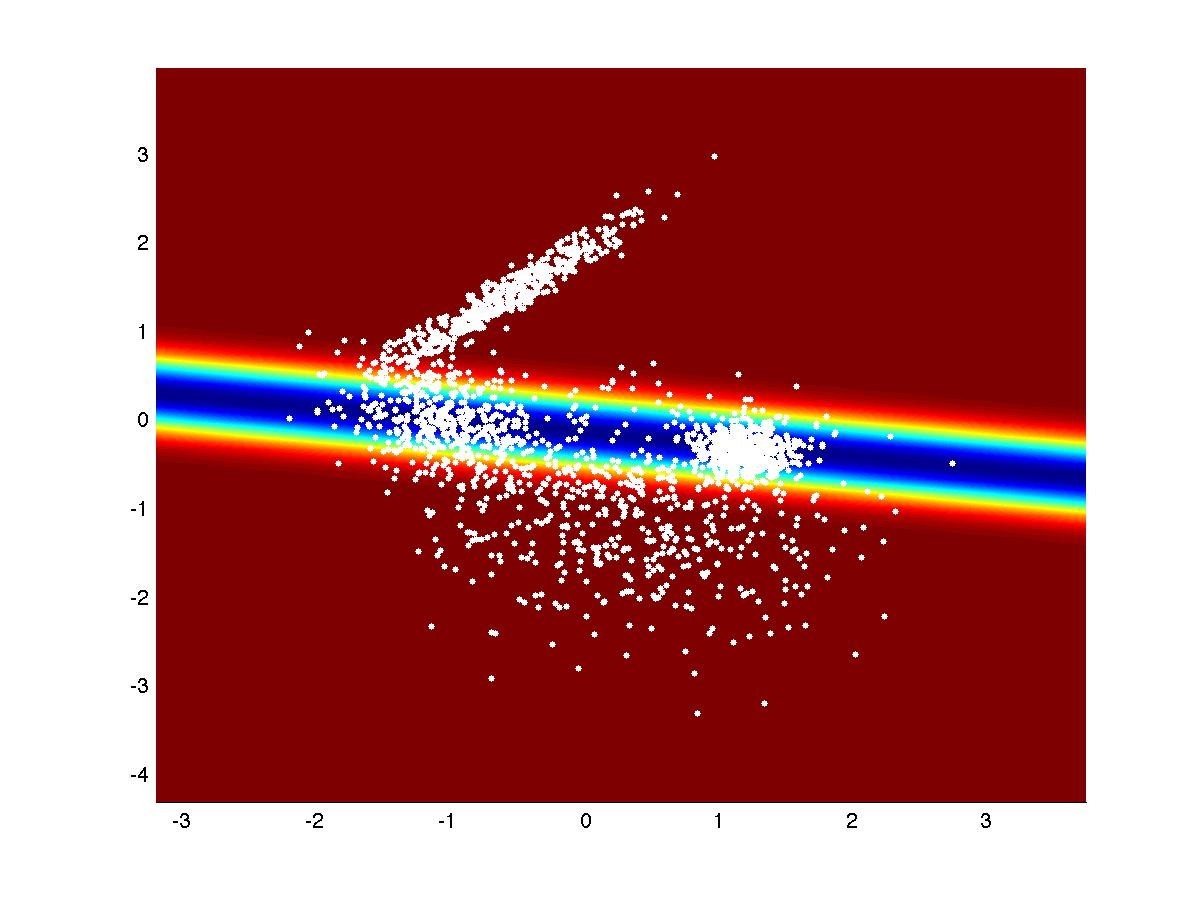
\includegraphics[trim = 150px 100px 150px 70px, clip=true,width=\textwidth]{VC1.jpg}
        \end{subfigure}
       
         \begin{subfigure}[b]{90 px}
                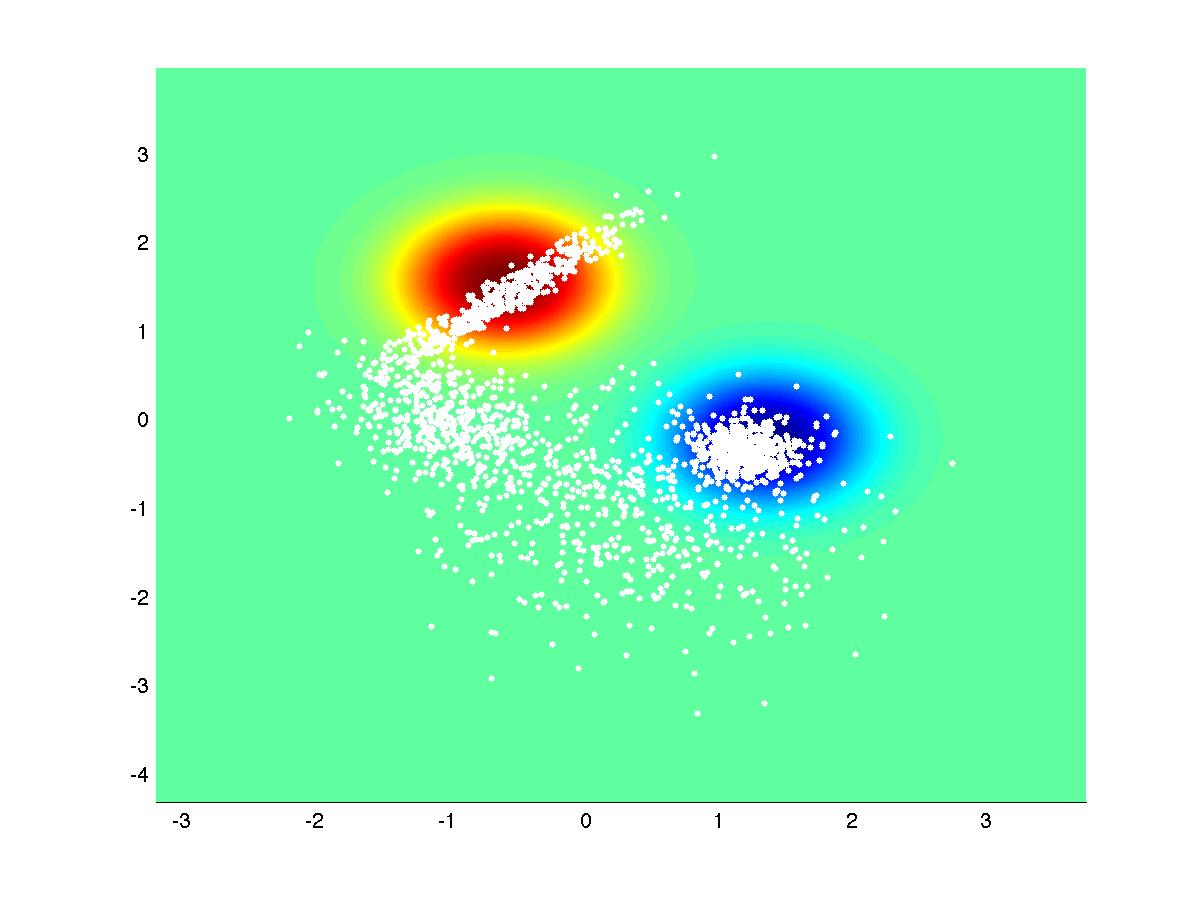
\includegraphics[trim = 150px 100px 150px 70px, clip=true,width=\textwidth]{global2.jpg}
        \end{subfigure}
        ~
         \begin{subfigure}[b]{90 px}
                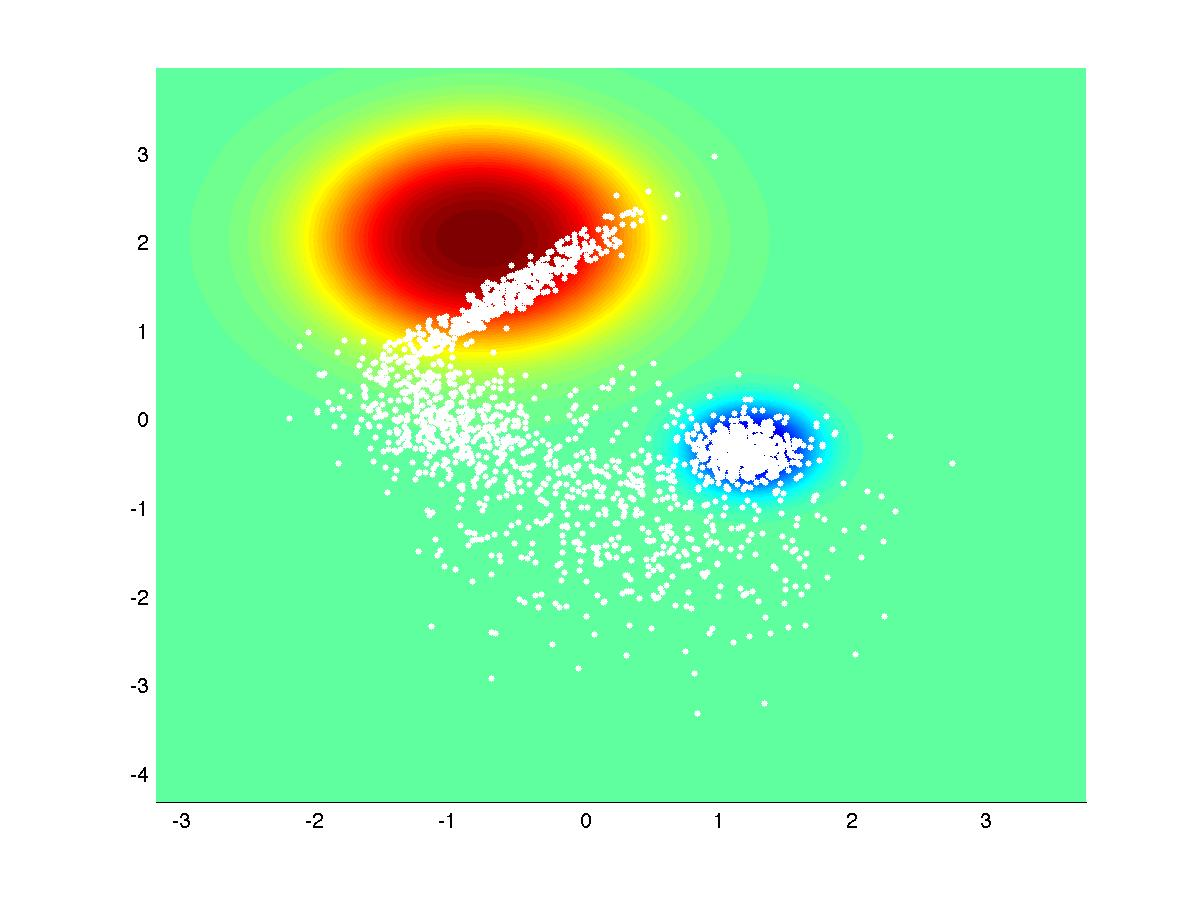
\includegraphics[trim = 150px 100px 150px 70px, clip=true,width=\textwidth]{VL2.jpg}
        \end{subfigure}
        ~
        \begin{subfigure}[b]{90 px}
                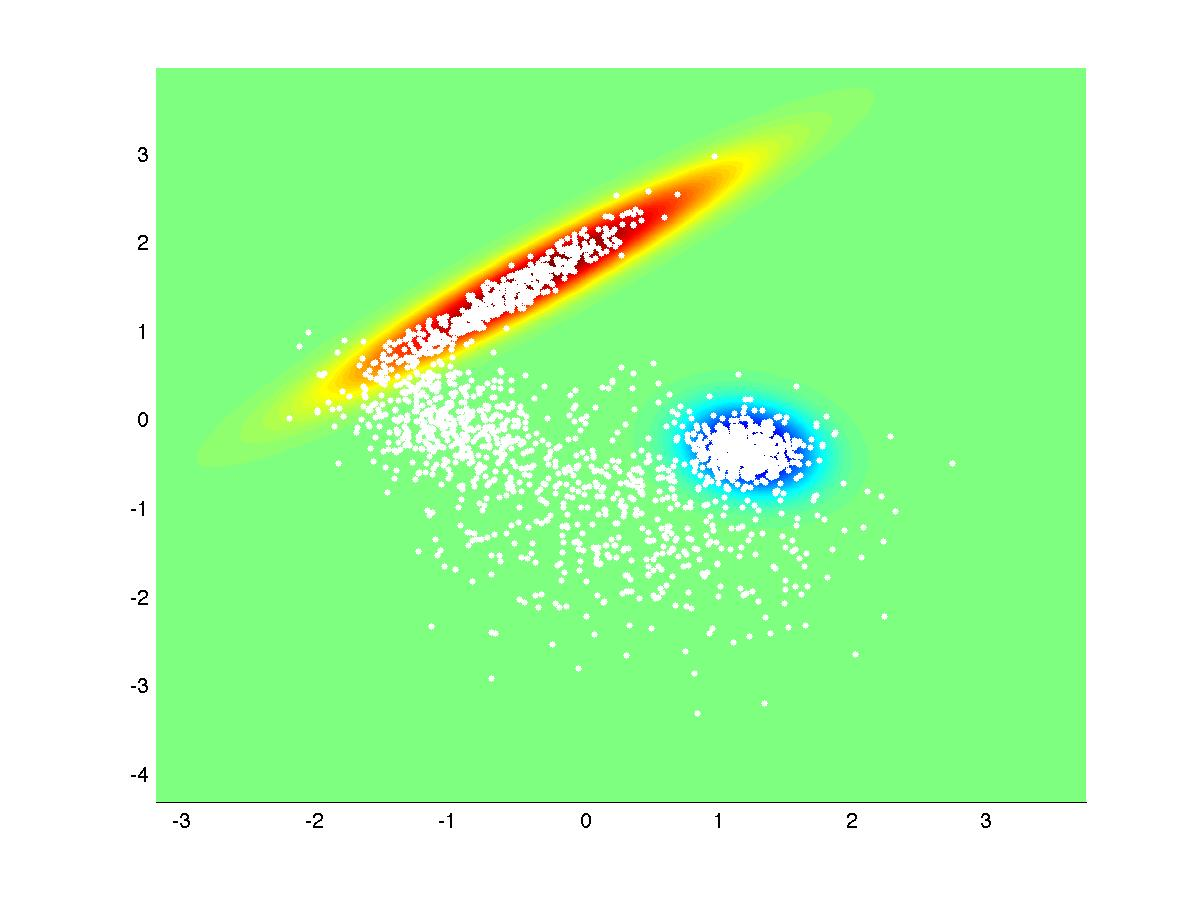
\includegraphics[trim = 150px 100px 150px 70px, clip=true,width=\textwidth]{VC2.jpg}
        \end{subfigure}
       
         \begin{subfigure}[b]{90 px}
                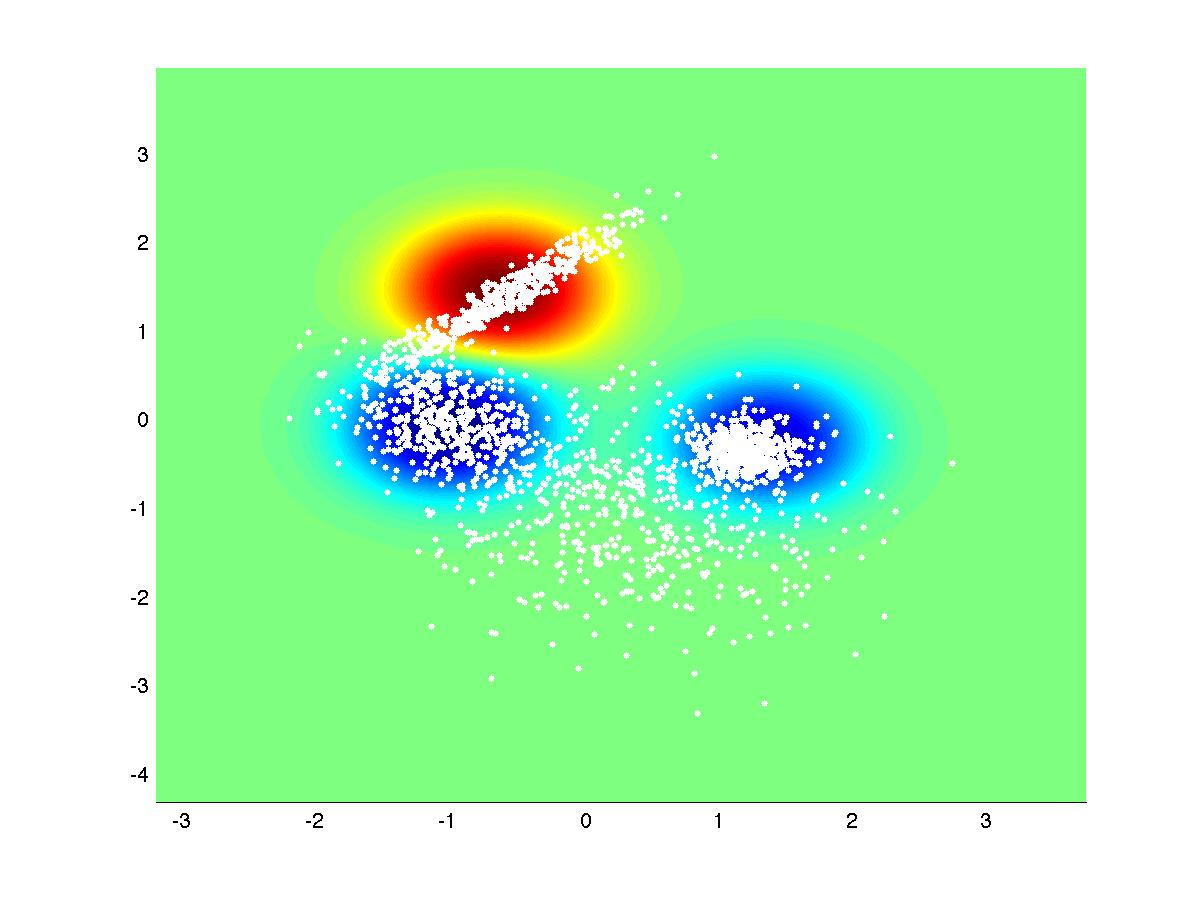
\includegraphics[trim = 150px 100px 150px 70px, clip=true,width=\textwidth]{global3.jpg}
        \end{subfigure}
        ~
         \begin{subfigure}[b]{90 px}
                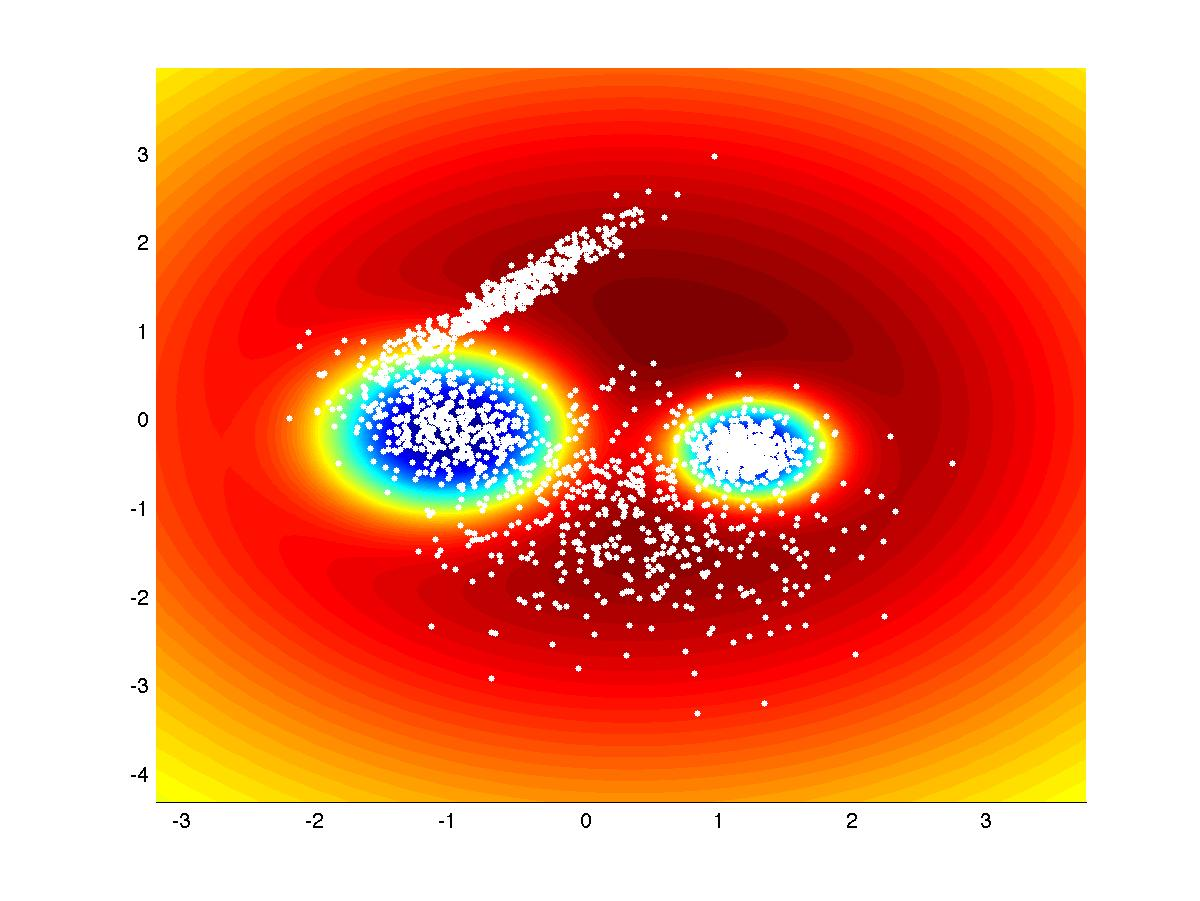
\includegraphics[trim = 150px 100px 150px 70px, clip=true,width=\textwidth]{VL3.jpg}
        \end{subfigure}
        ~
        \begin{subfigure}[b]{90 px}
                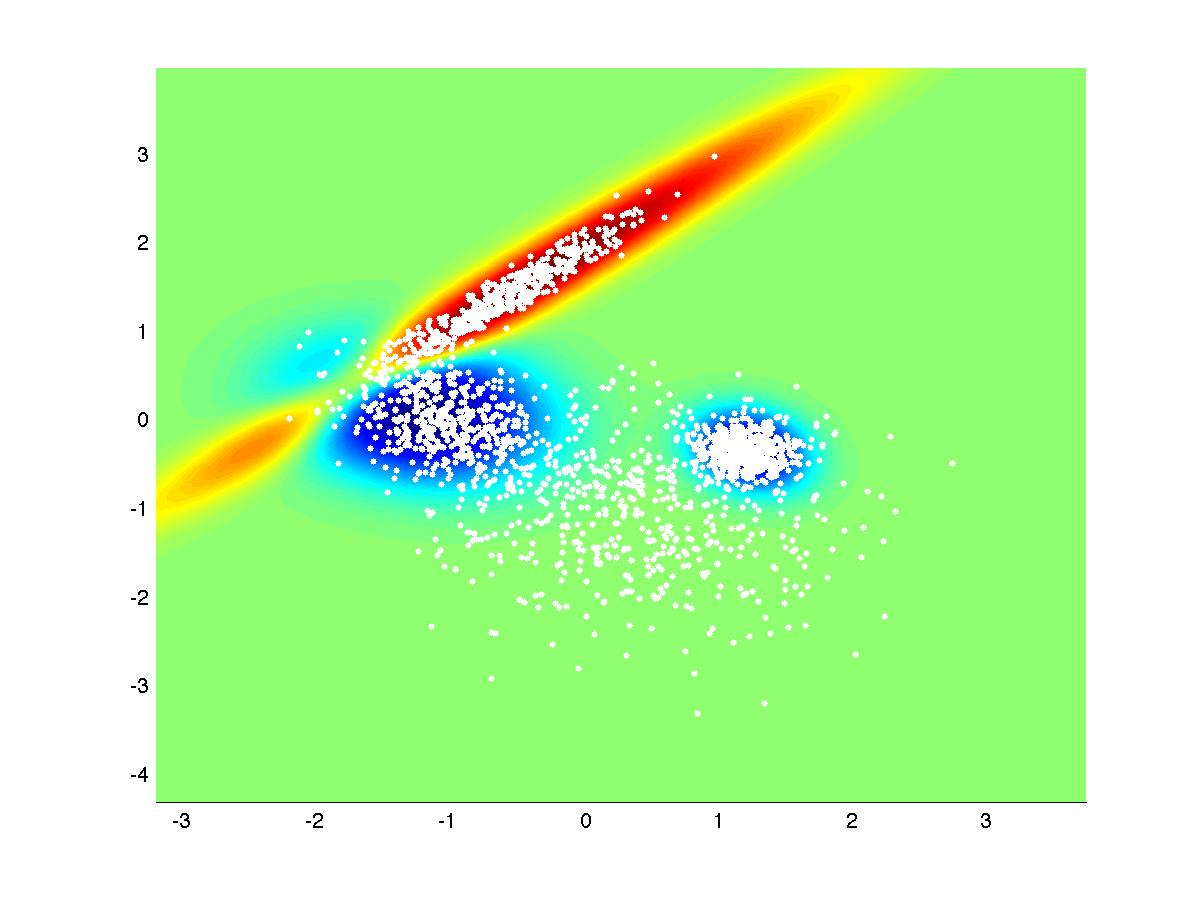
\includegraphics[trim = 150px 100px 150px 70px, clip=true,width=\textwidth]{VC3.jpg}
        \end{subfigure}
       
         \begin{subfigure}[b]{90 px}
                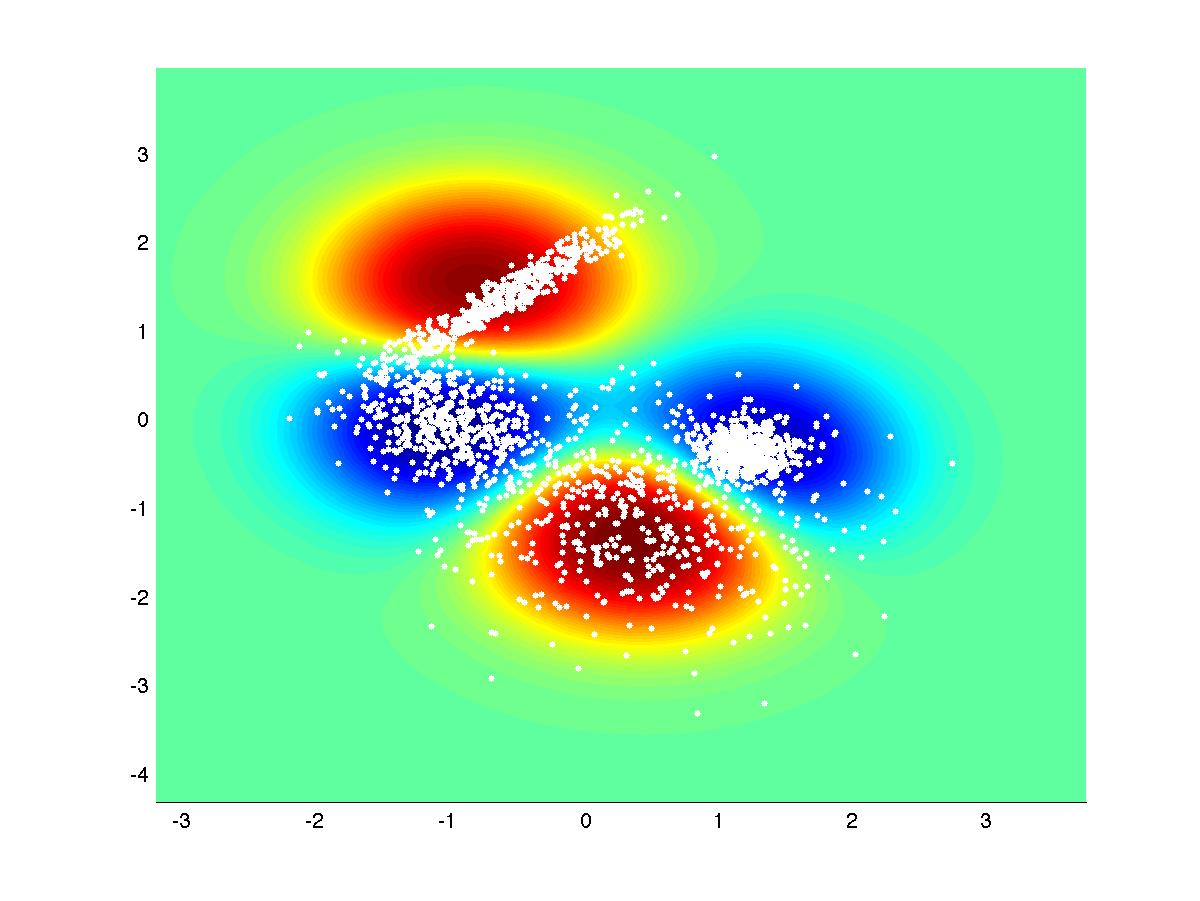
\includegraphics[trim = 150px 100px 150px 70px, clip=true,width=\textwidth]{global4.jpg}
                \caption{Global length scale}
        \end{subfigure}
        ~
         \begin{subfigure}[b]{90 px}
                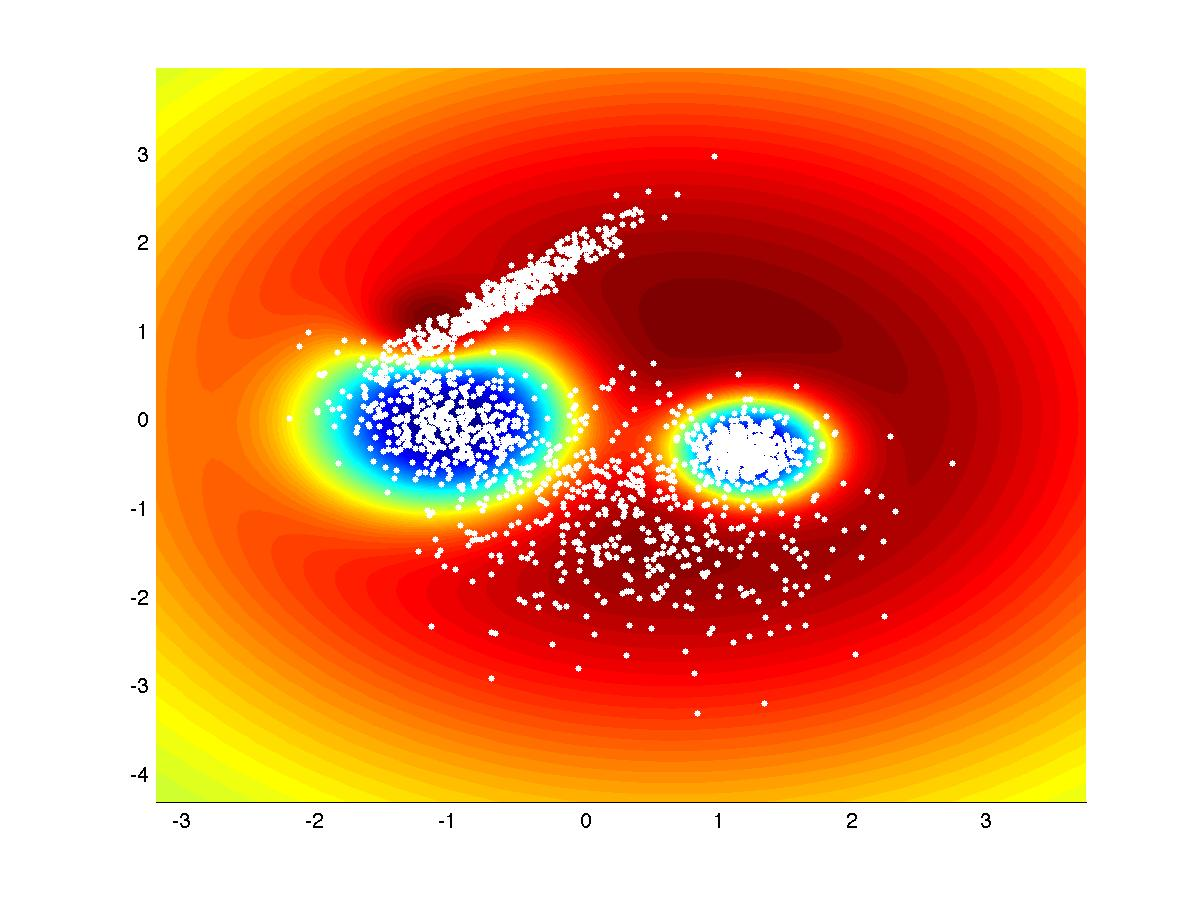
\includegraphics[trim = 150px 100px 150px 70px, clip=true,width=\textwidth]{VL4.jpg}
                \caption{Variable length scale}
        \end{subfigure}
        ~
        \begin{subfigure}[b]{90 px}
                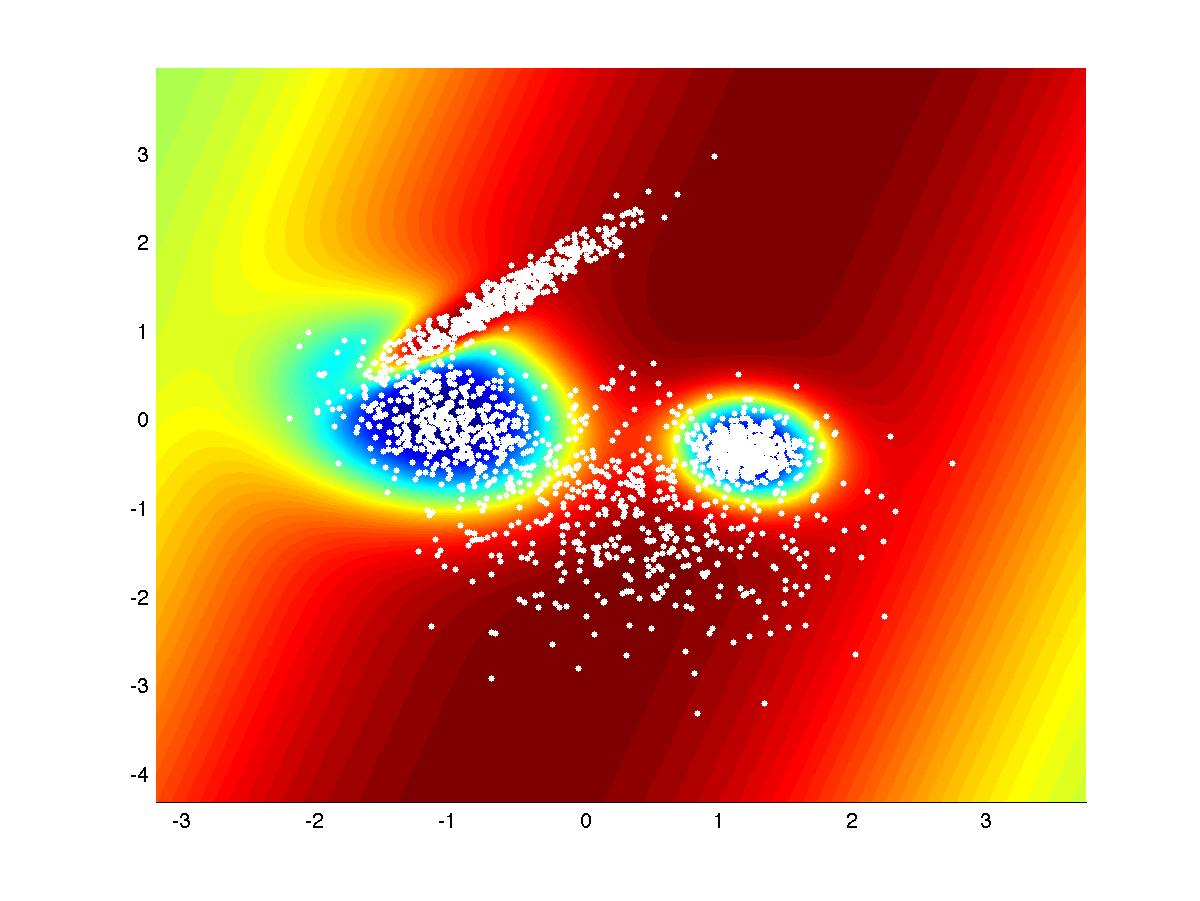
\includegraphics[trim = 150px 100px 150px 70px, clip=true,width=\textwidth]{VC4.jpg}
                \caption{Variable covariance}
        \end{subfigure}
               
        \caption{A comparisons between different sparse GP approaches with 1 to 4 bases functions using (a) a global length scale, (b) variable length scales and (c) variable covariances }
        \label{fig-toy-comparison}
\end{figure*}

\subsection{Linear Regression Prior}

GPs tend to perform well in interpolation but not as well in extrapolating. The regression function will fall back to the prior mean in areas where there is no training data. A common preprocessing technique is to subtract the mean of the output prior to training then adding it to the prediction of the model. Another way is to subtract a simple linear regression model and train the GP to learn the variation from that. This way, the GP will fall back to the linear regression prediction as a way of last resort instead of falling back to 0. We can incorporate this directly into the optimization objective instead of having it as a separate preprocessing step by redefining $K$ as concatenation of the linear and non-linear features, or in other words setting $K=[K|X|\underset{n}{1}]$. Furthermore, the regularization matrix in \eqref{eq-linear-regression-objective-rectangular} can be modified so that it penalizes for leaning high coefficients for the non-linear terms but no cost for learning linear terms by setting the corresponding elements in the diagonal of $I$ to 0, or the last $d+1$ elements. Therefore, as $\sigma_{n}^{2}$ goes to infinity, the model will get closer to a simple linear regression model.

\subsection{Sample Weighting and Bias Control}

So far the objective is to minimize the sum of squared errors, which is a suitable objective for most applications. However, this objective is naturally biased to the mean of the input and output distribution, therefore sacrificing data samples in less represented regions of space. This is not always a desired effect

\section{Other Objectives}
\label{sec-other-objectives}

\subsection{Minimizing the Maximum}
\subsection{Maximizing the number of fitting samples}

\section{Dataset Description}
\label{sec-dataset}

\section{Experiments and Results}
\label{sec-experiment}

\section{Conclusion}
\label{sec-conclusion}

\footnotesize{
\bibliographystyle{mn2e}
\bibliography{biblio.bib}	
}

\end{document}
